% This file was created by tikzplotlib v0.9.8.
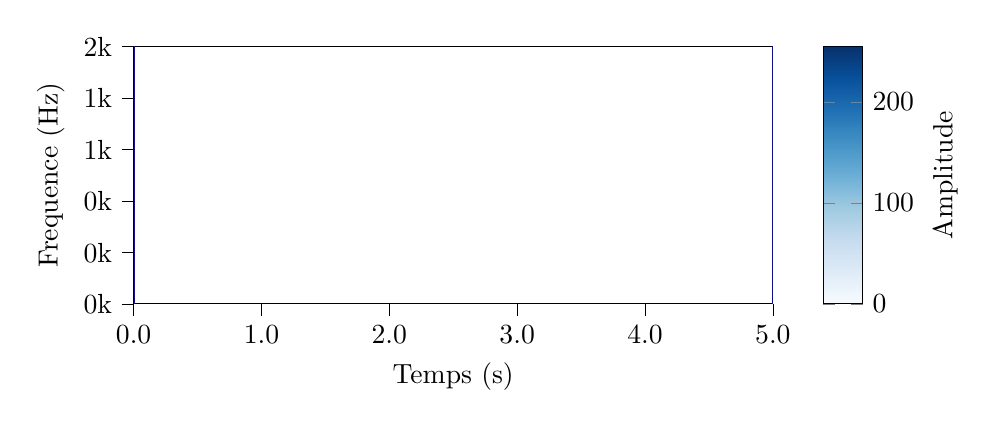
\begin{tikzpicture}

\begin{axis}[
colorbar,
colorbar style={ylabel={Amplitude}},
colormap={mymap}{[1pt]
  rgb(0pt)=(0.968627450980392,0.984313725490196,1);
  rgb(1pt)=(0.870588235294118,0.92156862745098,0.968627450980392);
  rgb(2pt)=(0.776470588235294,0.858823529411765,0.937254901960784);
  rgb(3pt)=(0.619607843137255,0.792156862745098,0.882352941176471);
  rgb(4pt)=(0.419607843137255,0.682352941176471,0.83921568627451);
  rgb(5pt)=(0.258823529411765,0.572549019607843,0.776470588235294);
  rgb(6pt)=(0.129411764705882,0.443137254901961,0.709803921568627);
  rgb(7pt)=(0.0313725490196078,0.317647058823529,0.611764705882353);
  rgb(8pt)=(0.0313725490196078,0.188235294117647,0.419607843137255)
},
height=0.4\linewidth,
point meta max=255,
point meta min=2.18132037129633e-07,
tick align=outside,
tick pos=left,
width=.8\linewidth,
x grid style={white!69.0196078431373!black},
xlabel={Temps (s)},
xmin=-0.5, xmax=249.5,
xtick style={color=black},
xtick={249.5,199.5,149.5,99.5,49.5,-0.5},
xticklabels={5.0,4.0,3.0,2.0,1.0,0.0},
y grid style={white!69.0196078431373!black},
ylabel={Frequence (Hz)},
ymin=0, ymax=43.975,
ytick style={color=black},
ytick={0,8.795,17.59,26.385,35.18,43.975},
yticklabels={0k,0k,0k,1k,1k,2k}
]
\addplot graphics [includegraphics cmd=\pgfimage,xmin=-0.5, xmax=249.5, ymin=879.5, ymax=-0.5] {ponderation1-010.png};
\end{axis}

\end{tikzpicture}
